\section{Cadre du pfe}
\begin{figure}[H]
  \center
  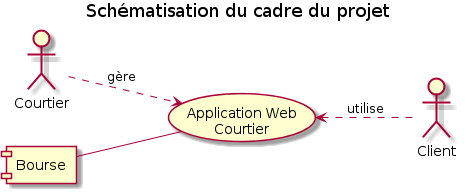
\includegraphics[scale=0.7]{../graph/schemaProjet.png}
\end{figure}

Après avoir décrit les différentes notions importantes dans le cadre de notre projet, nous pouvons définir l'environnement, ou plus exactement la position dans laquelle on place chaque acteur.\\

On considère que la personne qui fourni l'application Web (nous) est un courtier (ou broker en anglais). C'est également lui qui fourni les accès, mise à jour, etc. \\

Le joueur quant à lui sera un client du courtier. Il utilise l'application afin d'accéder à différentes informations sur son portefeuille et aussi pour le consituer. De plus, le joueur n'accède pas directement à la bourse puisqu'il passe par l'intermédiaire de l'application, donc du courtier, pour y accéder. Il aura donc accès à une 'sous'-bourse qui sera définie par le courtier lui-même.